\documentclass[technote,a4paper,leqno]{IEEEtran}
\pdfoutput=1

% packages
\usepackage[utf8]{inputenc}
\usepackage[T1]{fontenc}
\usepackage{amsmath,amssymb}
\usepackage[pdftex]{graphicx}
\usepackage{caption}
\usepackage[hang]{subfigure}
\captionsetup{format=hang}
\usepackage{url}
\usepackage[super]{nth}
\usepackage{nicefrac}
\usepackage[breaklinks]{hyperref}
\def\UrlBreaks{\do\/\do-}
\usepackage[absolute,overlay]{textpos}
\usepackage{tikz}
\usetikzlibrary{shapes, calc, shapes, arrows, snakes}
\usepackage{csquotes}
\usepackage{booktabs}  % for \toprule, \midrule and \bottomrule
\usepackage{pbox}
\usepackage{braket} % needed for nice printing of sets
\usepackage[english]{babel}
\usepackage{mathtools}
\usepackage{xspace}
\usepackage[inner=2.5cm,outer=2.5cm,top=2.5cm,bottom=2cm,includeheadfoot]{geometry}
% \usepackage{glossaries}
% \loadglsentries[main]{glossary}
% \makeglossaries

\usepackage[nameinlink, noabbrev,capitalise]{cleveref} % has to be after hyperref, nthe l.137 ...eam attr{/N 4}  file{sRGBIEC1966-2.1.icmorem, amsthm


% List stuff
\usepackage{enumitem}
\crefname{problemnr}{\textup{problem}}{\textup{problems}}
\newlist{problemnr}{enumerate}{1}
\setlist[problemnr]{label={P\arabic*}, ref=P\arabic*}
\crefalias{problemnri}{problemnr}

\newcommand*{\eg}{e.g.\@\xspace}


\usepackage[binary-units,group-separator={,}]{siunitx}
\sisetup{per-mode=fraction,
         binary-units=true,
         group-separator = {\,},
         range-phrase=-}
\DeclareSIUnit\pixel{px}
\usepackage{microtype}

\DeclareGraphicsExtensions{.jpg}
\DeclareMathOperator{\sgn}{sgn}
\DeclareMathOperator*{\minimize}{minimize}
\DeclareMathOperator*{\maximize}{maximize}

\newcommand\independent{\protect\mathpalette{\protect\independenT}{\perp}}
\def\independenT#1#2{\mathrel{\rlap{$#1#2$}\mkern2mu{#1#2}}}

\newcommand{\titleboth}{Semantische Segmentierung mit Deep Learning}
\title{\titleboth}
\author{%
\makebox[.4\linewidth]{Marvin Teichmann\thanks{\IEEEauthorrefmark{1} These authors contributed equally to this work.}\IEEEauthorrefmark{1}}% ORCID: http://orcid.org/0000-0002-9178-2970
\and \makebox[.4\linewidth]{Martin Thoma\IEEEauthorrefmark{1}}} % ORCID: http://orcid.org/0000-0002-6517-1690

\hypersetup{
    pdfauthor   = {Martin Thoma},
    pdfkeywords = {semantic segmentation, pixelwise classification, pixel-level classification},
    pdfsubject  = {Segmentation},
    pdftitle    = {\titleboth},
}

\begin{document}
\maketitle
%!TEX root = vorlage.tex

\begin{abstract}
Distinguishing medical instruments from background is a basic task which
supplements many applications and further analysis. If this task works robust
and fast, one can think about instance segmentation of medical instruments,
operation phase detection, pose estimation of the instruments, recognition of
the organs and ill tissue.

This work is part of a practical at KIT.
\end{abstract}


%!TEX root = vorlage.tex

\section{Introduction}\label{sec:introduction}
Operations like the removal of a tumor or the gallbladder (a cholecystectomy)
require the body of the patient to be opened. However, minimal-invasive
operations got more and more attentions since~1987~\cite{wickham1987new}. In
this kind of operation, the surgeon tries to make as little and as small cuts
in the patients body as possible. The advantage is that the patients skin can
heal faster and thus the patient can recover faster from the damage which was
done by the operation. The disadvantage of minimal-invasive operations is that
the operation itself gets harder for the surgeon. Special medical equipment has
to be used: Small cameras and fiber optic cables so that the surgeons can see
what their doing, % TODO: http://health.stackexchange.com/q/7304/2445

Machines can not only provide the possibility to make more fine-grained
movements (e.g. with the \textit{da Vinci} Surgical System (Intuitive Surgical,
Mountain View, Calif)), but also improve vision. For example, the limited
visibility due to cautarization-induced smoke can be fought by highlighting the
medical instruments, the instruments themselves can be recognized and the
operation phase can be detected. If the camera images had a pixel-wise
segmentation of medical instruments and background, those tasks would be
simpler.

%!TEX root = vorlage.tex

\section{Related Work}\label{sec:related-work}

Pixel-wise segmentation was successfully applied in other domains. For example,
\cite{bittel2015pixel} introduces a system which does pixel-wise segmentation
for autonomous cars of the classes \textit{street} and \textit{no street}. A
more detailed introduction to semantic segmentation can be found
in~\cite{thoma2016survey}.

An early example of semantic segmentation in medicine
is~\cite{wei1997automatic}. The authors suggested to place a marker on the
instrument which can easily be distinguished from background just by color. The
problem with this approach is that existing medical instruments can not easily
be colored due to costly approval procedures. Hence a semantic segmentation
algorithm which works with existing medical instruments is necessary.

For example, in~\cite{allan2013toward} the authors detected and localized
surgical instruments in laparoscopic images to estimate the pose of the
instrument in 3D. They used Random Forests.



% TODO: Wo in der Medizininformatik?

%!TEX root = vorlage.tex

\section{Models}

In this practical, we were examining deep neural network models for semantic
segmentation. The most basic neural network model is a so called
\textit{multilayer Perceptron} (\textit{MLP}). MLPs consist of an input layer,
multiple hidden layers and an output layer. Each layer consists of nodes. The
number of nodes of the input layer is determined by the features and the number
of output nodes is determined by the classes. The number of nodes in the hidden
layers can be arbitrary large, but is typically between 0.25 and 3 times the
number of the layer before. The parameters which get adjusted during the
training of a model are called \textit{weights}. One weight is between two
neurons of neighboring layers.

Each node has an activation function. Two functions which are used very often
are the \textit{sigmoid function} and the \textit{rectified linear function}.

The sigmoid activation function is

\[\varphi: \mathbb{R} \rightarrow (0, 1) \qquad \varphi(x) = \frac{1}{1 + e^{-x}}\]

while rectified linear units (commonly abbreviated with ReLU) have the
activation function

\[\varphi: \mathbb{R} \rightarrow [0, \infty) \qquad \varphi(x) = \max(0, x)\]

A more detailed introduction to MLPs can be found in~\cite{Mitchell1997}.

\subsection{Convolutional Neural Networks}
One of the most important extensions of MLPs are so called
\textit{Convolutional Neural Networks} (CNNs). Those introduce two new layer types
besides the fully connected layers: convolutional layers and pooling layers.
Each convolutional layer has $k \in \mathbb{N}_{\geq 1}$ filters of size $p
\times p \times c$, where $p \in \mathbb{N}_{\geq 1}$ is a design choice and $c
\in \mathbb{N}_{\geq 1}$ is the number of channels of the layer before. The
input layer has typically three channels: Red, green, blue (RGB). When $k$
filters get applied in layer $A$, then the output of layer $A$ has $k$
channels.\\
The parameters which get adjusted during training in convolutional layers are
the weights of the filters. A layer with $k$ filters of size
$p \times p \times c$ has $k \cdot p^2 \cdot c$ weights which get adjusted.

Convolutions produce an output which is smaller than their input, as one can see
in~\cref{fig:convolution-size}.

\begin{figure}[ht]
    \centering
    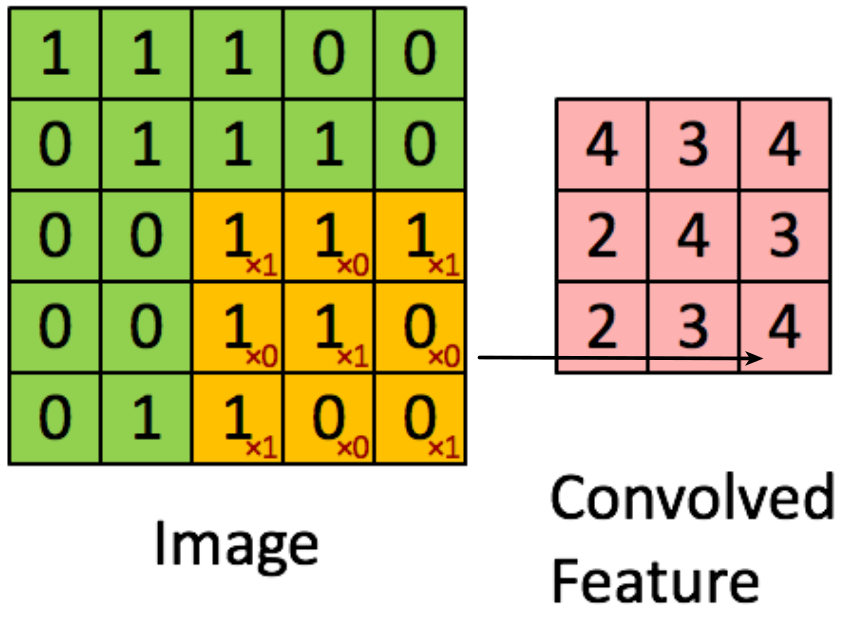
\includegraphics[width=\linewidth]{images/convolution-schematic.png}
    \caption{A $5 \times 5$ image convolved with a $3 \times 3$ filter becomes
             a $3 \times 3$ image as the filter size minus one gets removed
             from the input image size.\\
             Image source:~\cite{Cyfoo}}
    \label{fig:convolution-size}
\end{figure}

Sometimes it is desired to get an output of the same size as the input. In this
case the image is padded with $\frac{\text{filter size} - 1}{2}$ in each
direction. Commonly, the padding is done with zeroes.

The pooling layers do not learn any parameter. They reduce the data being
processed by the network by grouping it. Pooling layers have four hyperparameters:
the pooling function, the pooling size, the strides and the border mode.
The pooling size gives the size of the region to which the pooling function
gets applied. Typically, $3 \times 3$ pooling is chosen. For those four~pixels
the maximum function is chosen. Another option is average pooling. The stride
is the parameter which reduces the amount of processed data. A stride of $(2, 2)$
is used which has the effect of reducing the data to $\nicefrac{1}{4}$th of
the original amount.

There are a couple of well-known image classification networks for which both,
the architecture and the weights are available. One of those networks is called
VGG-16 (for \textit{Visual Geometry Group})~\cite{KarenSimonyan,simonyan2014very}.


\subsection{Fully Convolutional Neural Networks}

Fully Convolutional Networks (FCNs) were introduced by~\cite{long2015fully}.
They were shown to improve performance in semantic segmentation tasks over
standard convolutional neural networks (CNNs).

FCNs combine four ideas:

\begin{enumerate}
    \item Train an image classification network for $k$ classes,
    \item interpret this network as $k$ filters of a single, non-linear
          convolution,
    \item apply those filters to images of arbitrary size to receive a
          coarse heat map for the $k$ classes.
    \item Finally, train an upsampling network to get a fine-grained semantic
          segmentation.
\end{enumerate}

Upsampling is realized by padding and convolution as visualized
in~\cref{fig:upsampling}. It is worth emphasizing that this upsampling is
learned.

\begin{figure}[ht]
    \centering
    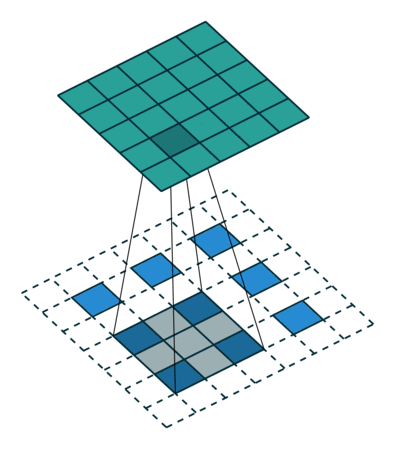
\includegraphics[width=\linewidth]{images/upsampling2-16.png}
    \caption{Upsampling: The blue input gets padded by the white cells. Then
             a convolution is applied --- visualized in gray --- to produce
             the green output.\\
             Image source:~\cite{vdumoulin2016}}
    \label{fig:upsampling}
\end{figure}


%!TEX root = vorlage.tex

\section{Experiments}\label{sec:experiments}

A desktop computer with a Titan Black and an Intel Core i7-4930K was used for
the training of the model and its evaluation.

%!TEX root = vorlage.tex

\subsection{The data}

The experiments were done on the \textit{Instrument segmentation and tracking}
dataset of the Endoscopic Vision Challenge
\enquote{EndoVis}\footnote{\href{http://endovis.grand-challenge.org/}{http://endovis.grand-challenge.org}}.
It contains photos of minimal-invasive operations. The dataset already contains
a training-test-split. The training data consists of four operations. Each
operation has 40~RGB~images in a resolution of $\SI{640}{\pixel} \times
\SI{480}{\pixel}$. The test set has 10~more images of those 4~operations as
well as 50~images for 2~more operations. This means, in total the training data
consist of $4 \cdot 40 = 160$ photos and the testing contains $4 \cdot 10 + 2
\cdot 50 = 140$ photos. As each pixel has to be classified as \textit{medical
instrument} or \textit{background}, there are
$140 \cdot 640 \cdot 480 = \num{43008000}$ classifications to be done for
testing.

The training data consist of $\SI{90.5}{\percent}$ background
($\SI{90.8}{\percent}$ in the testing data); the remaining pixels are medical
instruments. This means an accuracy of $\SI{90.8}{\percent}$ can be reached
without looking at the test image.

Analyzing the data, one can also see that some positions in the image are more
likely than others to contain a medical instrument. This is visualized
in~\cref{fig:medical-instrument-positions}.

\begin{figure}[ht]
    \centering
    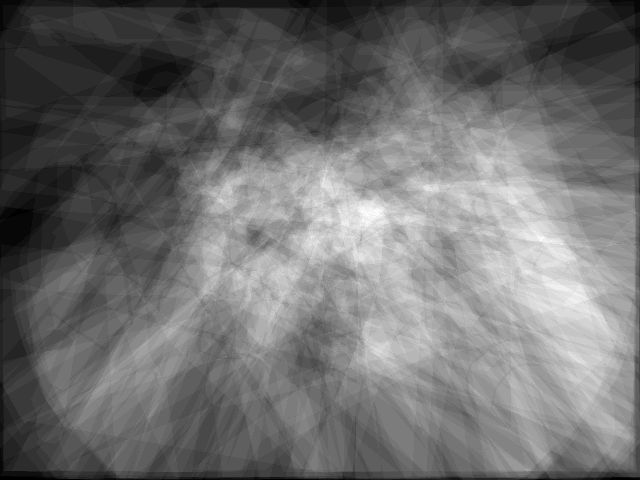
\includegraphics[width=\linewidth]{images/instrument-positions.png}
    \caption{Position of medical instruments in the training data.
             The brighter the color, the more often was a medical instrument
             at this position. One can clearly see that the borders contain
             medical instruments less often. Also, in the center they are much
             more often.}
    \label{fig:medical-instrument-positions}
\end{figure}

%!TEX root = vorlage.tex

\subsection{Base line experiments}\label{sec:ap3}

The most basic information for pixel-wise semantic segmentation is the color of
the pixel. Typically, images are in RGB format. This means the image has
three~channels ({\color{red} R}ed, {\color{green} G}reen, {\color{blue} B}lue).
Each channel has 8~bit and thus $2^8 = 256$ possible values, ranging from 0 to
255. This gives ${(2^8)}^3 = \num{16777216}$ possible colors for each pixel.
Obviously, only the color can not give a perfect result in all circumstances as
the measured color changes due to smoke, shadows, specular~highlights and
insufficient illumination. But it gives an impression how important local
features are for the specific problem.

A model with 64~sigmoid nodes in a first hidden layer with $\SI{50}{\percent}$
dropout~\cite{srivastava2014dropout}, 64~ReLu nodes in a second hidden layer
with $\SI{50}{\percent}$ dropout and one sigmoid output unit was used as a
baseline.

The architecture of the baseline model is visualized
in~\cref{fig:baseline-architecture}. Neither preprocessing nor data
augmentation were applied.

The baseline model achieved a pixel-wise accuracy
of~$\SI{92.88}{\percent}$,\footnote{This is the same as the DICE coefficient.}
a precision of $\SI{76.13}{\percent}$ and a recall of $\SI{32.94}{\percent}$.
The confusion matrix is given in~\cref{table:cm-model-301}.

\begin{figure}[ht]
    \centering
        \newcommand{\width}{0.2}
    
\tikzset{sigmoid/.style={path picture= {
    \begin{scope}[x=1pt,y=10pt]
      \draw plot[domain=-7:7] (\x,{1/(1 + exp(-\x))-0.5});
    \end{scope}
    }
  }
}

\tikzset{relu/.style={path picture= {
    \begin{scope}[x=7pt,y=6pt]
      \draw plot[domain=-1:0] (\x,0);
      \draw plot[domain=0:1] (\x,\x);
    \end{scope}
    }
  }
}

\tikzstyle{input}=[draw,fill=red!50,circle,minimum size=20pt,inner sep=0pt]
\tikzstyle{hidden}=[draw,fill=white,circle,minimum size=20pt,inner sep=0pt]
\tikzstyle{output}=[draw,fill=white,circle,minimum size=20pt,inner sep=0pt]
\tikzstyle{bias}=[draw,dashed,fill=gray!50,circle,minimum size=20pt,inner sep=0pt]
\tikzstyle{layer}=[fill=gray!70]

\tikzstyle{stateTransition}=[->, thick]

\begin{tikzpicture}[scale=2,yscale=0.6]
    \fill[layer] (  -\width,-1.9) rectangle (  \width,1.9);
    \fill[layer] (1+-\width,-1.9) rectangle (1+\width,1.9);
    \fill[layer] (2+-\width,-1.9) rectangle (2+\width,1.9);
    \fill[layer] (3+-\width,-1.9) rectangle (3+\width,1.9);
    \node (l1label) at  (0, -2.1) {3};
    \node (l2label) at  (1, -2.1) {64};
    \node (l3label) at  (2, -2.1) {64};
    \node (l4label) at  (3, -2.1) {1};
    \node (r)[input,fill=red]   at (0, 1) {R};
    \node (g)[input,fill=green] at (0, 0) {G};
    \node (b)[input,fill=blue]  at (0,-1) {B};

    \node (h11)[hidden, sigmoid] at (1, 1.5) {};
    \node (h12)[hidden, sigmoid] at (1, 0.5) {};
    \node[circle, inner sep=0] (h13) at (1,-0.5) {\vdots};
    \node (h14)[hidden, sigmoid] at (1,-1.5) {};
    \node (h21)[hidden, relu] at (2, 1.5) {};
    \node (h22)[hidden, relu] at (2, 0.5) {};
    \node[circle, inner sep=0] (h23) at (2,-0.5) {\vdots};
    \node (h24)[hidden, relu] at (2,-1.5) {};

    \node (o1)[output, sigmoid] at (3,0) {};

    \draw[stateTransition] (r) -- (h11) node [midway,above=-0.06cm] {};
    \draw[stateTransition] (r) -- (h12) node [midway,above=-0.06cm] {};
    \draw[stateTransition] (r) -- (h13) node [midway,above=-0.06cm] {};
    \draw[stateTransition] (r) -- (h14) node [midway,above=-0.06cm] {};
    \draw[stateTransition] (g) -- (h11) node [midway,above=-0.06cm] {};
    \draw[stateTransition] (g) -- (h12) node [midway,above=-0.06cm] {};
    \draw[stateTransition] (g) -- (h13) node [midway,above=-0.06cm] {};
    \draw[stateTransition] (g) -- (h14) node [midway,above=-0.06cm] {};
    \draw[stateTransition] (b) -- (h11) node [midway,above=-0.06cm] {};
    \draw[stateTransition] (b) -- (h12) node [midway,above=-0.06cm] {};
    \draw[stateTransition] (b) -- (h13) node [midway,above=-0.06cm] {};
    \draw[stateTransition] (b) -- (h11) node [midway,above=-0.06cm] {};

    \draw[stateTransition] (h11) -- (h21) node [midway,above=-0.06cm] {};
    \draw[stateTransition] (h11) -- (h22) node [midway,above=-0.06cm] {};
    \draw[stateTransition] (h11) -- (h23) node [midway,above=-0.06cm] {};
    \draw[stateTransition] (h11) -- (h24) node [midway,above=-0.06cm] {};
    \draw[stateTransition] (h12) -- (h21) node [midway,above=-0.06cm] {};
    \draw[stateTransition] (h12) -- (h22) node [midway,above=-0.06cm] {};
    \draw[stateTransition] (h12) -- (h23) node [midway,above=-0.06cm] {};
    \draw[stateTransition] (h12) -- (h24) node [midway,above=-0.06cm] {};
    \draw[stateTransition] (h13) -- (h21) node [midway,above=-0.06cm] {};
    \draw[stateTransition] (h13) -- (h22) node [midway,above=-0.06cm] {};
    \draw[stateTransition] (h13) -- (h23) node [midway,above=-0.06cm] {};
    \draw[stateTransition] (h13) -- (h24) node [midway,above=-0.06cm] {};
    \draw[stateTransition] (h14) -- (h21) node [midway,above=-0.06cm] {};
    \draw[stateTransition] (h14) -- (h22) node [midway,above=-0.06cm] {};
    \draw[stateTransition] (h14) -- (h23) node [midway,above=-0.06cm] {};
    \draw[stateTransition] (h14) -- (h21) node [midway,above=-0.06cm] {};

    \draw[stateTransition] (h21) -- (o1) node [midway,above=-0.06cm] {};
    \draw[stateTransition] (h22) -- (o1) node [midway,above=-0.10cm] {};
    \draw[stateTransition] (h23) -- (o1) node [midway,above=-0.06cm] {};
    \draw[stateTransition] (h24) -- (o1) node [midway,above=-0.06cm] {};

    \draw [
    thick,
    decoration={
        brace,
        mirror,
        raise=0.5cm
    },
    decorate
] (1+-\width, -1.8) -- (2+\width, -1.8)
node [pos=0.5,anchor=north,yshift=-0.55cm] {50\% dropout};
\end{tikzpicture}
    \caption{Architecture of the baseline model.}
    \label{fig:baseline-architecture}
\end{figure}

%!TEX root = vorlage.tex

\subsection{Local Models}\label{sec:ap4}

A slightly better model than the baseline used the coordinate of the pixel in
the image as two additional features ($x, y \in \mathbb{R}$) as well as
$\SI{3}{\pixel}$ erosion and dilation. This is known as a morphological
opening. This model achieved an higher accuracy and a higher precision, but the
recall improved most. As one can see in the results
in~\cref{table:results-local-model-experiments}, most of the improvement is due
to the coordinate features. The confusion matrix is given
in~\cref{table:cm-model-303}.

\begin{table}[ht]
    \centering
    \begin{tabular}{lrrr}
    \toprule
    Model              & Accuracy & Precision & Recall \\\midrule
    Baseline (BL)      & $\SI{92.88}{\percent}$  & $\SI{76.13}{\percent}$ & $\SI{32.94}{\percent}$\\
    BL + CFs           & $\SI{93.42}{\percent}$  & $\underline{\SI{76.98}{\percent}}$ & $\SI{40.65}{\percent}$\\
    BL + Opening       & $\SI{91.07}{\percent}$  & $\SI{74.76}{\percent}$ & $\SI{4.50 }{\percent}$\\
    BL + CFs + Opening & $\underline{\SI{93.51}{\percent}}$  & $\SI{76.76}{\percent}$ & $\underline{\SI{42.30}{\percent}}$\\
    \bottomrule
    \end{tabular}
    \caption{Results of the local model experiments. The coordinate features (CFs)
             improved the quality.}
    \label{table:results-local-model-experiments}
\end{table}

An example for the segmentation can be seen
in~\cref{fig:model-303-segmentation}. The model fits some of the edges of the
medical instruments very well, but has severe problems with specular
highlights. It is also not able to deal with the red reflection on the medical
instruments head and very dark, but not black areas with little image
information.

\begin{figure}[t]
    \centering
    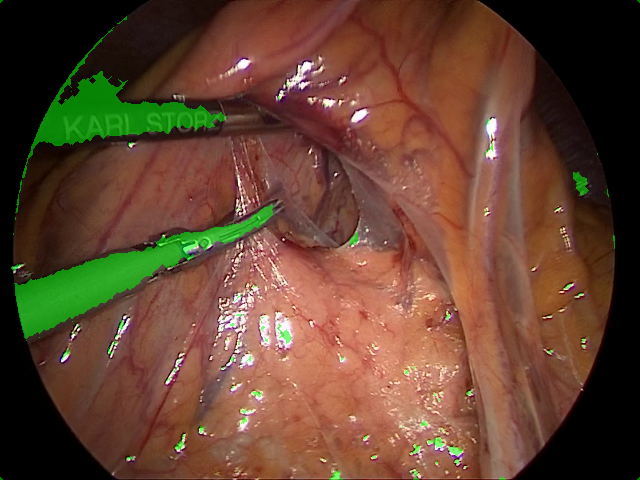
\includegraphics[width=\linewidth]{images/model-303-img_06_raw-overlay.png}
    \caption{Example segmentation by the local model with opening.}
    \label{fig:model-303-segmentation}
\end{figure}

Astonishingly, the accuracy of models which made use of a tiny patch around the
pixel which was to classify decreased to about $\SI{92.11}{\percent}$, the
precision is $\SI{42.30}{\percent}$ and the recall is $\SI{76.74}{\percent}$.
The classification of one image took about $\SI{1.54}{\second}$. In theory, the
model could simply set the weights to 0 and thus ignoring the other features.
This means such a model should never be worse than a model without the
surrounding pixel information. Besides programming errors and numerical
problems, the problem might be the increased number of parameters. It is
possible that the optimization was stuck in a local minimum.



%!TEX root = vorlage.tex

\subsection{Fully Convolutional Networks}\label{sec:ap5}

\subsubsection{Architecture}
In the following, the mean value of the image net dataset was subtracted from
each image channel (mean blue: 103.939, mean green: 116.779, mean red: 123.68).

For the following experiment, the VGG-16 architecture as introduced
in~\cite{simonyan2014very} was used. Not only was the architecture used, but
the network was also pre-trained on image net and used as described
in~\cite{Fossard2016}. The VGG-16 architecture consists of 20~layers:

\begin{enumerate}
    \item \verb+conv1_1+, \verb+conv1_2+, \verb+pool1+: Two convolutional
          layers with 64~filters of size $3 \times 3$ each, followed by max
          pooling with a stride of $s = (2, 2)$ and a pooling region of
          $p = (2, 2)$.
    \item \verb+conv2_1+, \verb+conv2_2+, \verb+pool2+: Two convolutional
          layers with 128~filters of size $3 \times 3$ each, followed by max
          pooling with a stride of $s = (2, 2)$ and a pooling region of
          $p = (2, 2)$.
    \item \verb+conv3_1+, \verb+conv3_2+, \verb+conv3_3+, \verb+pool3+: Three
          convolutional layers with 256~filters of size $3 \times 3$ each,
          followed by max pooling with a stride of $s = (2, 2)$ and a pooling
          region of $p = (2, 2)$.
    \item \verb+conv4_1+, \verb+conv4_2+, \verb+conv4_3+, \verb+pool4+: Three
          convolutional layers with 512~filters of size $3 \times 3$ each,
          followed by max pooling with a stride of $s = (2, 2)$ and a pooling
          region of $p = (2, 2)$.
    \item \verb+conv5_1+, \verb+conv5_2+, \verb+conv5_3+, \verb+pool5+: Three
          convolutional layers with 512~filters of size $3 \times 3$ each,
          followed by max pooling with a stride of $s = (2, 2)$ and a pooling
          region of $p = (2, 2)$.
    \item \verb+fc6+: A fully connected layer with 4096~nodes.
    \item \verb+fc7+: A fully connected layer with 1000~nodes.
\end{enumerate}

The network was trained on image net data. The idea is to use the general
image recognition features learned in the first layers. Thus the network is a
very sophisticated preprocessing algorithm.
% The layer \verb+fc7+ is discarded
% and the feature vector produced by \verb+fc6+ is used.

After \verb+fc7+, a convolutional layer \verb+score_fr+ with $k$ filters of the
shape $1 \times 1 \times 1000$ is added where $k$ is the number of classes.
Then an upscore layer \verb+up+ is added to scale the coarse output of
\verb+score_fr+ to the same size as the input image.

The $k=2$ upsampling filters of size $64 \times 64$ were initialized as a
bilinear upsampling. Those filters make the result so consistent. As they
mainly interpolate between neighboring pixels, they will never give
unrealistically small segments.

The FCN was trained end-to-end with the mean softmax cross entropy
between logits and labels as training objective:

\[- \frac{1}{|D|} \sum_{(\mathbf{x}, \mathbf{y}) \in D} \sum_{y_i \in \mathbf{y}} \left [ y_i \ln a_i + (1-y_i) \ln(1 - a_i)\right ]\]

where $D$ is the set of training data, $x$ is a feature vector, $y$ is a one-hot
encoded target and $a_i$ is the prediction for the $i$-th class of the classifier.

Each weight was regularized with L2 loss. This means the original objective
function $f_\text{training data}(\mathbf{w})$ which gets minimized was modified
to

\[\tilde{f}_\text{training data}(\mathbf{w}) = f_\text{training data}(\mathbf{w}) + \sum_{w \in \mathbf{w} w^2}\]
\clearpage
Not only the given training data was used, but it was also heavily augmented by
the following methods:

\begin{itemize}
    \item Horizontal flipping
    \item Vertical flipping
    \item Horizontal and vertical flipping
    \item Random brightness adjustments
    \item Random crops were taken
\end{itemize}

\subsubsection{Results}
The FCN evaluation results are shown in \cref{table:challenge-results}. Our
fully convolutional network is noticeably better than the other semantic
segmentation systems.

A training run with 5000 epochs took about 5.5 hours. Running the network on a
single image takes in average $\SI{1.3}{\second}$.


\subsubsection{Analysis of data augmentation}

Data augmentation is commonly done to train the network to become invariant to
changes in the data which should not matter. For example, in computer vision
this is an image-wide change in brightness.

Data augmentation becomes especially useful if very little data is present to
artificially increase the available training material. However, it is unclear
how much data is enough data and which data augmentation methods have which
effect on the quality of the semantic segmentation system.

We were interested in three properties: The quality of the segmentation system
at the end of \num{10000} epochs (11 hours) of training, the stability of the
quality during training and the speed of convergence.

To evaluate the quality of the training, four metrics were used and evaluated
on the test set after each 250~epochs:

\begin{itemize}
    \item Accuracy: $\frac{TP + TN}{TP + TN + FP + FN} \in [0, 1]$
    \item Precision: $\frac{TP}{TP + FP} \in [0, 1]$
    \item Recall: $\frac{TP}{TP + FP} \in [0, 1]$
    \item F1-Score: $2 \frac{\text{Precision} \cdot \text{Recall}}{\text{Precision} + \text{Recall}} \in [0, 1]$
\end{itemize}

Other metrics besides the accuracy were used as over \SI{90}{\percent} of the
data was background. Precision and recall are typical choices to solve this
problem. We thought about using the F1 score as a single number is always
simpler to compare than two numbers. However, for our experiments with FCNs on
this dataset the Person correlation coefficient of the accuracy and the F1
score is 0.96. The F1 score has lower values and a higher variance, but it
shows the same characteristics for FCNs on this datasets.

\Cref{fig:graph-accuracy-all} suggests that data augmentation has little to no
effect on the overall accuracy. Only random crops seem to have a negative
effect on accuracy.

\Cref{fig:graph-precision-all,fig:graph-recall-all} show that the precision
and recall have a lot of variance for all data augmentation methods. Random
crops seem to have a negative effect on precision and recall as well.

All training methods suffer from enormous outliers in the quality even during
late stages in the training.

We did not notice any effect of any data augmentation method on the stability
during the training.


%!TEX root = vorlage.tex

\section{Discussion}\label{sec:discussion}

Fully Convolutional Networks are also in this domain clearly superior to
traditional approaches. However, examining results such as the one shown
in~\cref{fig:fcn-result}, one can see that there is room for improvement. While
the overall position was correctly detected and the proposal is fairly
consistent, the model fails to match borders exactly. Simple improvements such
as combining the results of a FCN with the baseline might already fix this
problem. More elaborate techniques such as Conditional Random Fields (CRFs) are
also promising.

\begin{figure}[ht]
    \centering
    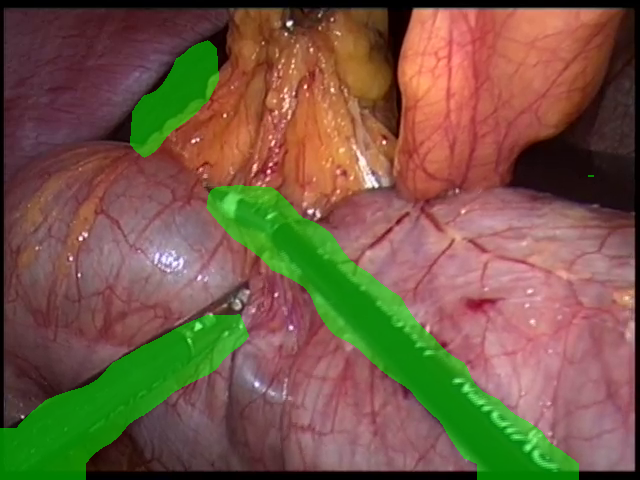
\includegraphics[width=\linewidth]{images/7-img_07.png}
    \caption{Semantic segmentation result of the FCN. While it }
    \label{fig:fcn-result}
\end{figure}

%!TEX root = vorlage.tex

\section{Acknowledgement}\label{sec:acknowledgement}

We would like to thank the \enquote{Begabtenstiftung Informatik Karlsruhe} for
supporting our research. They supported the work on TensorVision
(\href{https://github.com/TensorVision/TensorVision}{github.com/TensorVision/TensorVision}),
which was used for this practical.
% (\href{https://www.informatik.kit.edu/begabtenstiftung_informatik_karlsruhe.php}{www.informatik.kit.edu/begabtenstiftung\_informatik\_karlsruhe.php})

\bibliography{literature}
\bibliographystyle{IEEEtranSA}\vfill
% \columnbreak
% \printglossaries%

%!TEX root = vorlage.tex

\clearpage\onecolumn
\begin{appendices}
\section{Tables}

\begin{table}[ht]
    \centering
    \begin{tabular}{llrr}
    \toprule
    ~                & ~ & \multicolumn{2}{c}{\textbf{Predicted class}}\\
    ~                & ~ & \multicolumn{1}{c}{\textbf{0}} & \multicolumn{1}{c}{\textbf{1}} \\% \cmidrule{3-4}
    \textbf{Actual}  & \multicolumn{1}{c}{\textbf{0}} & \num{38640407}  & \num{2654875} \\
    \textbf{class}   & \multicolumn{1}{c}{\textbf{1}} &   \num{408816}  & \num{1303902} \\ \bottomrule
    \end{tabular}
    \caption{Confusion matrix of a model trained soley on pixel colors.
             Class~0 is background, class~1 is medical instruments.}
    \label{table:cm-model-301}
\end{table}

\begin{table}[ht]
    \centering
    \begin{tabular}{llrr}
    \toprule
    ~                & ~ & \multicolumn{2}{c}{\textbf{Predicted class}}\\
    ~                & ~ & \multicolumn{1}{c}{\textbf{0}} & \multicolumn{1}{c}{\textbf{1}} \\% \cmidrule{3-4}
    \textbf{Actual}  & \multicolumn{1}{c}{\textbf{0}} & \num{38989042}  & \num{3780484} \\
    \textbf{class}   & \multicolumn{1}{c}{\textbf{1}} &    \num{60181}  &  \num{178293} \\ \bottomrule
    \end{tabular}
    \caption{Confusion matrix of a model trained soley on pixel colors. Additionally,
             a morphological closing operation with $\SI{3}{\pixel}$ was applied.
             Class~0 is background, class~1 is medical instruments.}
    \label{table:cm-model-301-closing}
\end{table}

\begin{table}[ht]
    \centering
    \begin{tabular}{llrr}
    \toprule
    ~                & ~ & \multicolumn{2}{c}{\textbf{Predicted class}}\\
    ~                & ~ & \multicolumn{1}{c}{\textbf{0}} & \multicolumn{1}{c}{\textbf{1}} \\% \cmidrule{3-4}
    \textbf{Actual}  & \multicolumn{1}{c}{\textbf{0}} & \num{38541570}  & \num{2284099} \\
    \textbf{class}   & \multicolumn{1}{c}{\textbf{1}} &   \num{507653}  & \num{1674678} \\ \bottomrule
    \end{tabular}
    \caption{Confusion matrix of a model trained on pixel colors and the pixels coordinates. Additionally, a morphological closing operation was applied.
             Class~0 is background, class~1 is medical instruments.}
    \label{table:cm-model-303}
\end{table}
\end{appendices}


\end{document}
